% Independent two-column proof. Compile with latexmk -pdf lcl-proof.tex.
\documentclass[sigconf,nonacm]{acmart}
\usepackage{stfloats}
\setcopyright{none}
\settopmatter{printacmref=false,printfolios=true}
\title{Safety and Liveness of Lock Chain Length Deadlock Detection}
% Use document-level metadata without publisher fields or build timestamps.
\makeatletter
\let\hyxmp@parse@acmart\relax
\let\hyxmp@embed@packet\relax
\makeatother
\pdfsuppressptexinfo=15
\pdfinfoomitdate=1
\pdftrailerid{}
\hypersetup{pdftitle={Safety and Liveness of Lock Chain Length Deadlock Detection},
  pdfsubject={Safety and conditional liveness of LCL and LCL+ distributed deadlock detection and resolution in OceanBase},
  hidelinks}

\newcommand{\lclv}{\mathrm{LCLV}}
\newcommand{\puid}{\mathrm{PuID}}
\newcommand{\prid}{\mathrm{PrID}}
\newcommand{\ap}{\mathrm{AP}}
\newcommand{\usg}{\mathrm{USG}}
\newcommand{\asg}{\mathrm{ASG}}
\newcommand{\dist}{\mathrm{Dist}}
\newcommand{\asgdist}{\mathrm{AsgDist}}
\newcommand{\asgwidth}{\mathrm{AsgWidth}}
\newcommand{\sccdiam}{\mathrm{SccDiam}}
\newcommand{\phead}[1]{\par\noindent\textsc{#1.}\enspace}

\begin{document}
\maketitle
\hypersetup{pdfcreator={LaTeX},
  pdfsubject={Safety and conditional liveness of LCL and LCL+ distributed deadlock detection and resolution in OceanBase}}
\pagestyle{plain}
\thispagestyle{plain}
\raggedbottom
\appendix
\section{Safety and Liveness Proofs}

Transactions waiting for row locks in OceanBase form a distributed
wait-for graph (WFG) in which a vertex may wait on multiple downstream
holders at once. Each vertex maintains a dynamic lock chain length value
(\(\lclv\)) and candidate victim identifier (\(\puid\)), exchanging
fixed-size metadata only with its immediate downstream neighbors.
Definitions~3.1--4.10, Lemmas~5.1, 5.4, 5.6--5.8, and~5.10,
Corollary~5.9, and Theorems~5.5 and~5.11 follow the numbering of
\emph{\(\text{LCL}^+\): a Lock Chain Length-based Distributed Deadlock
Detection and Resolution Service Built for OceanBase} by Zhenkun Yang,
Chen Qian, and colleagues~\cite{lclplus} (expanding~\cite{lcl}), while
Theorems~5.1a and~5.12 formalize Sections~5.1.1 and~5.1.2. Under the
protocol premises below, Theorem~5.1a establishes historical soundness
(no manslaughter of never-deadlocked transactions) and the \(N\)-cycle
victim bound under asynchronous, lossy, or reordered updates within each
period; Theorem~5.5, Lemma~5.10, and Theorem~5.11 establish
single-period isolation and unique victim selection in every topmost
strongly connected component; and Theorem~5.12 gives multi-period
liveness across chained deadlocks and \(\text{LCL}^+\) Stage~0
pre-proliferation. Section~\ref{sec:model} describes the scope of the
companion TLA+ specification.

\phead{Theorem 5.1a (Asynchronous safety)}%
\emph{Let \(G=(V,E)\) be a snapshot WFG containing \(N\) simple directed
cycles, where vertices and edges leave \(G\) only as victims are
terminated and no new wait edges arrive. Across any sequence of
detection periods in which period resets discard prior-period spread
messages, while within each period updates may be lost, duplicated,
reordered, or cut short by early phase switches:}
\begin{enumerate}
  \item[\emph{(a)}] \emph{Historical soundness (no manslaughter). Every
    vertex detected by Stage~0 or Stage~3 belongs to a simple directed
    cycle in \(G\) on which it holds the strictly largest abortion
    priority.}
  \item[\emph{(b)}] \emph{Per-cycle victim bound. At most \(N\) vertices
    are terminated in total; in particular, if \(G\) is acyclic
    (\(N=0\)), no vertex is ever terminated.}
\end{enumerate}

\subsection*{Protocol premises}
\begingroup\sloppy
\setlength{\parindent}{0pt}
\setlength{\parskip}{0.25\baselineskip}
\textbf{Wait-for graph and identifiers.}
A snapshot WFG is a finite directed graph \(G=(V,E)\) without self-loops:
an edge \(A\to B\) (\(A\neq B\)) means transaction \(A\) waits for a
resource held by \(B\) (Definition~3.1). Under strict two-phase locking,
a blocked transaction releases no locks until terminated, so its
outgoing wait-for edges persist while both endpoints remain active. We
write \(A\Rightarrow B\) if there exists a directed walk from \(A\) to
\(B\), taking \(A\Rightarrow A\) of length \(0\) (Definition~3.2);
\(\dist(A,B)\) is the minimum walk length when \(A\Rightarrow B\)
(Definition~3.5); and \(A\Leftrightarrow B\) holds when both
\(A\Rightarrow B\) and \(B\Rightarrow A\) (Definition~3.3). Each vertex
\(X\in V\) carries a fixed unique private identifier \(\prid(X)\) and
fixed injective abortion priority \(\ap(X)\) defining a strict total
order on \(V\) (if raw priorities can tie, \(\ap(X)\) denotes the
lexicographic pair \((\mathrm{raw\_AP}(X),\prid(X))\); the paper sets
\(\ap=\prid\) without loss of generality, Definitions~4.1 and~4.3).
Dynamically, \(X\) stores \(\lclv(X)\in\mathbb{N}\) (initially \(0\),
Definition~4.4) and \(\puid(X)\in V\) (initialized to \(\prid(X)\) at
the start of every detection period, with prior-period spread updates
discarded across the reset, Definition~4.2). For \(U\subseteq V\),
\(\max\{U.\lclv\}=\max(\{0\}\cup\{X.\lclv : X\in U\})\)
(Definition~4.5).

\textbf{Strongly connected components and annulus subgraphs.}
Equivalence under \(\Leftrightarrow\) partitions \(V\) into strongly
connected components~\cite{tarjan}. Throughout Section~5, an \emph{SCC}
denotes a \emph{nontrivial} strongly connected component---one whose
vertices lie on at least one directed cycle, and hence satisfy
\(|S|\ge 2\) since \(G\) has no self-loops (vertices outside cycles form
trivial singletons \(\{X\}\) in~\cite[\S3.2]{lclplus}). For an SCC \(S\),
its \emph{upstream subgraph} \(\usg(S)\) is the subgraph induced by
\(\{X\in V : \exists A\in S,\; X\Rightarrow A\}\) (Definition~3.6), and
its \emph{annulus subgraph} \(\asg(S)\) is the subgraph induced by
\(\usg(S)\setminus S\) (Definition~3.7). Note that \(S\subseteq\usg(S)\),
and any edge \(X\to Y\) with \(Y\in\usg(S)\) has \(X\in\usg(S)\); if
furthermore \(Y\in\asg(S)\), then \(X\in\asg(S)\) (otherwise \(X\in S\)
and \(Y\Rightarrow S\) would give \(Y\in S\)). For \(X\in S\),
\(\asgdist(X,S)=0\); for \(X\in\asg(S)\), \(\asgdist(X,S)\) is the
maximum \(m\ge 1\) such that \(m\) distinct vertices
\(C_m(=X),\allowbreak \dots,\allowbreak C_1\in\asg(S)\) and \(C_0\in S\)
form a walk \(C_m\to\cdots\to C_1\to C_0\) (Definition~3.8). When
well-defined, \(\asgwidth(S)\) is \(\max\{\asgdist(X,S) : X\in\usg(S)\}\)
and \(\sccdiam(S)\) is \(\max\{\dist(X,Y) : X,Y\in S\}\)
(Definitions~4.6 and~4.7).

\textbf{Stages 1--3 (\(\text{LCL}\): Proliferation, Spread, Detection).}
At the start of each period, every active vertex resets
\(X.\puid:=X.\prid\).
\emph{Stage~1 (Proliferation, Definition~4.8):} Applying proliferation
on \(A\to B\) sets \(B.\lclv:=\max(B.\lclv,A.\lclv+1)\), leaving
\(\puid\) unchanged.
\emph{Stage~2 (Spread, Definition~4.9):} Applying spread on \(A\to B\)
first sets \(B.\lclv:=\max(B.\lclv,A.\lclv)\); if then
\(B.\lclv=A.\lclv\) and \(A.\puid.\ap>B.\puid.\ap\), it sets
\(B.\puid:=A.\puid\) (Formula~1).
\emph{Deduction round (Definition~4.10):} One round of proliferation (or
spread) applies the stage's update to every active edge in \(E\) at
least once, in arbitrary order and multiplicity.
\emph{Stage~3 (Detection and resolution):} On edge \(A\to B\)
(\(A\neq B\)), vertex \(B\) is detected as victim if
\(B.\lclv=A.\lclv\) and \(B.\puid=A.\puid=B.\prid\). Terminating a
victim removes it and all its incident edges from \(G\).

\textbf{Stage~0 (\(\text{LCL}^+\) local pre-proliferation).}
Preceding or accompanying proliferation, Stage~0 initiates local
depth-first walks carrying the active path stack \(P=(v_1,\dots,v_k)\)
across same-server edges~\cite[\S4.7, Algorithm~2]{lclplus}. On a local
edge \(v_k\to B\): if \(B=v_j\) already appears on \(P\)
(\(1\le j\le k\)), the cycle suffix \(C=(v_j,\dots,v_k)\) is a local
cycle and Stage~0 selects \(\arg\max_{X\in C} X.\ap\) as victim (taking
the suffix from \(v_j\), rather than the entire stack from \(v_1\), is
essential when \(j>1\) so upstream stem vertices are never selected). If
\(B\) is local and not on \(P\), Stage~0 sets
\(B.\lclv:=\max(B.\lclv,v_k.\lclv+1)\) and extends \(P\) by \(B\). If
\(B\) resides on a remote server, Stage~0 queues
\(B.\lclv:=\max(B.\lclv,v_k.\lclv+1)\) to the remote LCL buffer without
forwarding \(P\).

\textbf{Scope and relation to OceanBase.}
OceanBase executes periodic proliferation and spread windows of fixed
wall-clock duration (\(1.4\,\text{s}\) default) with message buffering
and rate-limiting, integrating Stage~3 checks into incoming spread
updates without runtime knowledge of \(\asgwidth(S)\) or
\(\sccdiam(S)\)~\cite[\S4.6, \S7.1]{lclplus}. Theorem~5.1a proves safety
for this asynchronous, potentially under-provisioned execution;
Theorems~5.11 and~5.12 prove completeness and liveness when periods
deliver the round counts of Definition~4.10.
\par
\endgroup

\begin{figure*}[t]
  \centering
  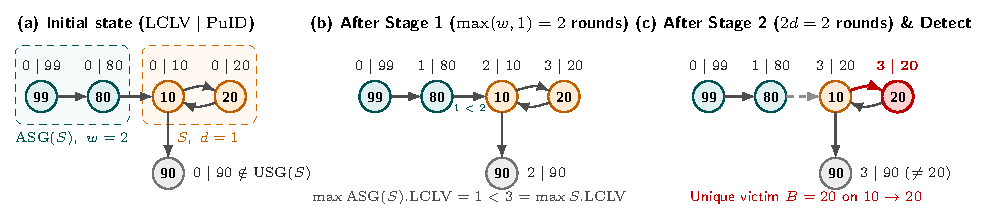
\includegraphics[width=0.96\textwidth]{figures/annulus-deduction.pdf}
  \caption{Representative execution of \(\text{LCL}\) on an SCC
  \(S=\{10,20\}\) (\(d=1\)) with a higher-priority upstream annulus chain
  \(\asg(S)=\{99,80\}\) (\(w=2\)) and a multi-outdegree downstream
  non-cycle neighbor \(90\notin\usg(S)\). Labels above vertices show
  \(\lclv\mid\puid\) (with \(\prid=\ap\)). After \(\max(w,1)=2\)
  proliferation rounds~(b), \(\asg(S)\) stabilizes strictly below \(S\),
  preventing \(99\) from entering \(S\) during spread~(c). Even under an
  interleaving where \(10\to 90\) raises \(90.\lclv\) to \(3\),
  \(90.\puid=90\neq 10.\puid=20\), so Stage~3 selects \(B=20\) uniquely.}
  \Description{Three panels showing initial state, state after two
  proliferation rounds, and state after two spread rounds on a five-node
  wait-for graph with annulus nodes 99 and 80, cycle nodes 10 and 20, and
  downstream node 90.}
  \label{fig:deduction}
\end{figure*}

\subsection{Asynchronous Safety}
\label{sec:async-safety}
\begin{proof}[Proof of Theorem 5.1a]
Consider first a victim \(v\) detected by Stage~0 when a local edge
\(v_k\to v_j\) closes a revisited suffix \(C=(v_j,\dots,v_k)\) of the
DFS stack. Because \(v_j,\dots,v_k\) are distinct and each step
\(v_r\to v_{r+1}\) and \(v_k\to v_j\) belongs to \(E\), \(C\) is a
simple directed cycle in \(G\), and Stage~0 selects
\(v=\arg\max_{X\in C} X.\ap\), which is strictly greater in \(\ap\) than
every \(X\in C\setminus\{v\}\).

Now consider any single period's Stage~1--3 execution (including inline
Stage~3 evaluation during Spread while earlier victims remove incident
edges). At period start, every active vertex \(X\) sets
\(X.\puid:=X.\prid\), so \(X.\puid.\ap=X.\ap\), and no stale spread
update from a prior period is applied. Stage~1 leaves \(\puid\)
untouched, and Stage~2 updates \(Y.\puid\) on a currently active edge
\(X\to Y\in E\) only when \(X.\puid.\ap>Y.\puid.\ap\), setting
\(Y.\puid:=X.\puid\). Fix a vertex \(v\). By induction on spread steps
within the period: \emph{(i)}~\(Y.\puid.\ap\) is strictly increasing
across every replacement of \(Y.\puid\) and hence always satisfies
\(Y.\puid.\ap\ge Y.\ap\), so no vertex can acquire \(v.\prid\) more than
once; and \emph{(ii)}~for each \(Y\neq v\) that ever acquires
\(Y.\puid=v.\prid\), recording the active edge \(p(Y)\to Y\in E\) of
that unique acquisition step gives that \(p(Y)\) already held
\(v.\prid\) at an earlier step of the period and
\[
  v.\ap \;=\; p(Y).\puid.\ap \;>\; Y.\puid.\ap \;\ge\; Y.\ap.
\]
Note that \(p(Y)\to Y\in E\) remains an edge of the initial graph \(G\)
even if \(p(Y)\) is later terminated during the period. Suppose active
edge \(u\to v\in E\) (\(u\neq v\)) triggers Stage~3 detection of \(v\),
so \(u.\puid=v.\puid=v.\prid\). Iterating \(p(\cdot)\) backward from
\(u\) steps strictly backward in acquisition time through vertices of
priority \(<v.\ap\) until reaching the sole initial holder \(v\),
yielding a simple directed path \(v=w_0\to w_1\to\cdots\to w_k=u\)
(\(k\ge 1\)) in \(G\) whose non-\(v\) vertices all satisfy
\(w_r.\ap<v.\ap\). Closing this path with \(u\to v\in E\) produces a
simple directed cycle \(C_v\) in \(G\) with
\(v=\arg\max_{X\in C_v} X.\ap\), proving~(a)---including for vertices
outside \(\usg(S)\) such as \(90\) in Figure~\ref{fig:deduction}.

For~(b), no vertex can be terminated twice because incident edges are
removed upon termination. Thus each terminated vertex \(v\) admits a
witness simple cycle \(C_v\) in \(G\) with
\(\max_{X\in C_v} X.\ap = v.\ap\). Because \(\ap\) is injective on \(V\),
\(v_1\neq v_2\) implies \(\max_{X\in C_{v_1}} X.\ap \neq
\max_{X\in C_{v_2}} X.\ap\), so \(C_{v_1}\neq C_{v_2}\). The map
\(v\mapsto C_v\) is therefore an injection from terminated vertices into
the \(N\) simple directed cycles of \(G\), bounding the total number of
terminations by \(N\).
\end{proof}

\subsection{Topmost SCC}
\label{sec:topmost}
\phead{Lemma 5.1}%
\emph{Suppose \(S_1\) and \(S_2\) are two SCCs in \(G\). If
\(\usg(S_1)=\usg(S_2)\), then \(S_1=S_2\).}
\begin{proof}
Pick any \(X\in S_1\) and \(Y\in S_2\). Since
\(X\in S_1\subseteq\usg(S_1)=\usg(S_2)\), there is \(Y'\in S_2\) with
\(X\Rightarrow Y'\); since \(Y',Y\in S_2\), \(Y'\Rightarrow Y\), so
\(X\Rightarrow Y\). Symmetrically, \(Y\in S_2\subseteq\usg(S_1)\) gives
\(Y\Rightarrow X\). Hence \(X\Leftrightarrow Y\) and \(S_1=S_2\).
\end{proof}

\noindent\textbf{Definitions 5.2 and 5.3.}\enspace
An SCC \(S_2\) is a \emph{proper upstream SCC} of an SCC \(S_1\) if
\(S_2\subseteq\asg(S_1)\). An SCC \(S\) is a \emph{topmost SCC} if it
has no proper upstream SCC.

\phead{Lemma 5.4}%
\emph{If \(S_2\) is a proper upstream SCC of \(S_1\), then
(i)~\(S_2\neq S_1\) and (ii)~\(\usg(S_2)\subsetneq\usg(S_1)\).}
\begin{proof}
By Definition~5.2 and Definition~3.7,
\(S_2\subseteq\asg(S_1)=\usg(S_1)\setminus S_1\), so
\(S_2\cap S_1=\varnothing\); since \(S_2\neq\varnothing\),
\(S_2\neq S_1\), giving~(i). For any \(X\in\usg(S_2)\), there exist
\(A\in S_2\) with \(X\Rightarrow A\) and, because
\(A\in S_2\subseteq\usg(S_1)\), \(B\in S_1\) with \(A\Rightarrow B\);
transitivity gives \(X\Rightarrow B\), so
\(\usg(S_2)\subseteq\usg(S_1)\). Equality is ruled out by~(i) and
Lemma~5.1, yielding \(\usg(S_2)\subsetneq\usg(S_1)\).
\end{proof}

\phead{Theorem 5.5}%
\emph{If \(G\) contains an SCC, then \(G\) contains at least one topmost
SCC.}
\begin{proof}
Suppose for contradiction that every SCC in \(G\) has a proper upstream
SCC. Starting from an SCC \(S_1\) with \(|\usg(S_1)|=n\), choose a
proper upstream SCC \(S_{k+1}\) of \(S_k\) for each \(k\ge 1\). By
Lemma~5.4(ii), \(|\usg(S_1)|>|\usg(S_2)|>\cdots\), so
\(|\usg(S_n)|\le 1\). Yet \(S_n\subseteq\usg(S_n)\) and every nontrivial
SCC satisfies \(|S_n|\ge 2\), a contradiction.
\end{proof}

\subsection{Annulus Subgraph}
\label{sec:annulus}
Throughout this subsection, fix a topmost SCC \(S\). Because \(S\) has
no proper upstream SCC, \(\asg(S)\) contains no directed cycle; hence
every walk inside \(\asg(S)\) visits distinct vertices of bounded length
\(\le |\asg(S)|\), so \(\asgdist(X,S)\) and \(\asgwidth(S)\) are finite.

\phead{Lemma 5.6}%
\emph{Let \(X_m\to X_{m-1}\to\cdots\to X_1\) be a walk of \(m\ge 1\)
distinct vertices in \(\asg(S)\). If \(X_{m+1}\in\asg(S)\) satisfies
\(X_{m+1}\to X_m\) (\(X_{m+1}\neq X_m\)), then
\(X_{m+1},X_m,\dots,X_1\) are \(m+1\) distinct vertices.}
\begin{proof}
If \(X_{m+1}=X_j\) for some \(1\le j\le m-1\), then
\(X_{m+1}\to X_m\to\cdots\to X_j(=X_{m+1})\) is a cycle of at least two
vertices entirely inside \(\asg(S)\). Its SCC would lie in \(\asg(S)\),
contradicting that \(S\) has no proper upstream SCC.
\end{proof}

\phead{Lemma 5.7}%
\emph{If \(X\in\asg(S)\) and \(Y\in\usg(S)\) satisfy \(X\to Y\)
(\(X\neq Y\)), then \(\asgdist(X,S)\ge\asgdist(Y,S)+1\).}
\begin{proof}
Let \(m=\asgdist(Y,S)\). If \(m=0\), then \(Y\in S\) and the walk
\(X\to Y\) witnesses \(\asgdist(X,S)\ge 1=m+1\). If \(m\ge 1\), then
\(Y\in\asg(S)\) and Definition~3.8 gives \(m\) distinct vertices
\(Y_m(=Y),Y_{m-1},\dots,Y_1\in\asg(S)\) and \(Y_0\in S\) with
\(Y_m\to\cdots\to Y_1\to Y_0\). By Lemma~5.6, \(X,Y_m,\dots,Y_1\) are
\(m+1\) distinct vertices in \(\asg(S)\), so
\(X\to Y_m\to\cdots\to Y_0\) witnesses \(\asgdist(X,S)\ge m+1\).
\end{proof}

\phead{Lemma 5.8}%
\emph{For every \(X\in\asg(S)\), let \(m=\asgdist(X,S)\). Then \(m\ge 1\),
and along any witnessing walk \(X_m(=X)\to X_{m-1}\to\cdots\to X_1\to X_0\)
with distinct \(X_m,\dots,X_1\in\asg(S)\) and \(X_0\in S\), we have
\(\asgdist(X_j,S)=j\) for all \(j\in\{0,1,\dots,m\}\).}
\begin{proof}
Since \(X_0\in S\), \(\asgdist(X_0,S)=0\). Applying Lemma~5.7 to each
edge \(X_j\to X_{j-1}\) (\(1\le j\le m\)) gives
\[
  \asgdist(X_j,S)\;\ge\;\asgdist(X_{j-1},S)+1,
\]
whence by induction \(\asgdist(X_j,S)\ge j\) and
\(\asgdist(X_m,S)\ge\asgdist(X_j,S)+(m-j)\). Since
\(\asgdist(X_m,S)=m\), the latter bound gives \(\asgdist(X_j,S)\le j\),
so \(\asgdist(X_j,S)=j\) for all \(0\le j\le m\).
\end{proof}

\phead{Corollary 5.9}%
\emph{For every \(X\in\asg(S)\), there exists \(Y\in\usg(S)\) with
\(X\to Y\) (\(X\neq Y\)) and \(\asgdist(X,S)=\asgdist(Y,S)+1\).}
\begin{proof}
Apply Lemma~5.8 to \(X=X_m\) and set \(Y=X_{m-1}\).
\end{proof}

\subsection{Cycle Detection and Resolution}
\label{sec:resolution}
Consider a fixed active graph \(G_k\) at the entry to Stage~1 with
arbitrary current labels \(L_0:X\mapsto X.\lclv\in\mathbb{N}\) (allowing
any values left by prior periods or \(\text{LCL}^+\) Stage~0). For a
topmost SCC \(S\) of \(G_k\), because \(\asg(S)\) is finite and acyclic
and every predecessor in \(G_k\) of any \(Y\in\asg(S)\) also lies in
\(\asg(S)\), the DAG fixed-point recurrence
\[
  H(Y)\;=\;\max\bigl(\{L_0(Y)\}\cup\{H(X)+1 : X\to Y\text{ in }G_k\}\bigr)
\]
is uniquely well-defined on \(\asg(S)\). Initially \(Y.\lclv=L_0(Y)\le
H(Y)\) holds unconditionally for every \(Y\in\asg(S)\), and every
subsequent proliferation or spread step on \(G_k\) preserves
\(Y.\lclv\le H(Y)\) by induction.

\phead{Lemma 5.10}%
\emph{Let \(S\) be a topmost SCC of \(G_k\) with \(w=\asgwidth(S)\).
From any initial \(\lclv\) assignment \(L_0\) at Stage~1 entry, after
\(\max(w,1)\) or more rounds of Stage~1 proliferation deductions on
\(G_k\):}
\begin{enumerate}
  \item[\emph{(i)}] \emph{the \(\lclv\) of every vertex in \(\asg(S)\) is
    fixed at \(H(X)\) and invariant under any further proliferation or
    spread steps on \(G_k\);}
  \item[\emph{(ii)}] \emph{for every \(X\in\asg(S)\) and \(Y\in\usg(S)\)
    with \(X\to Y\), \(X.\lclv < Y.\lclv\); and}
  \item[\emph{(iii)}] \emph{\(\max\{\asg(S).\lclv\} < \max\{S.\lclv\}\).}
\end{enumerate}
\begin{proof}
If \(\asg(S)=\varnothing\), then \(w=0\), (i) and (ii) hold vacuously,
and \(\max\{\asg(S).\lclv\}=0\) by Definition~4.5. Since \(|S|\ge 2\),
\(S\) contains at least one edge \(A\to B\); in round~1 of
proliferation, applying \(A\to B\) sets \(B.\lclv\ge A.\lclv+1\ge 1\),
so \(\max\{S.\lclv\}\ge 1 > 0\), establishing~(iii).

Now suppose \(\asg(S)\neq\varnothing\), so \(w\ge 1\). Partition
\(\asg(S)\) into \(S_j=\{X\in\asg(S):\asgdist(X,S)=j\}\) for
\(j=1,\dots,w\); by Lemma~5.8, each \(S_j\) is nonempty. We show by
induction on \(k\in\{0,1,\dots,w-1\}\) that after \(k\) proliferation
rounds, every \(Y\in S_{w-k}\) satisfies \(Y.\lclv=H(Y)\) and never
changes thereafter. If \(Y\in S_{w-k}\) has no incoming edge in \(G_k\)
(which holds for every \(Y\in S_w\) at \(k=0\) by Lemma~5.7, as well as
any shorter-branch source), then \(Y.\lclv\) never changes and already
equals \(L_0(Y)=H(Y)\). Otherwise \(k\ge 1\), and every predecessor
\(X\to Y\) lies in \(\asg(S)\) with \(\asgdist(X,S)\ge w-k+1=w-(k-1)\)
by Lemma~5.7, so \(X\in\bigcup_{r=0}^{k-1} S_{w-r}\). By the induction
hypothesis, every such \(X.\lclv\) is already fixed at \(H(X)\) before
round~\(k\) begins. Because \(Y\) enters round~\(k\) with
\(Y.\lclv\ge L_0(Y)\), round~\(k\) applies proliferation on every
incoming edge \(X\to Y\) at least once, and \(Y.\lclv\le H(Y)\),
\(Y.\lclv\) reaches \(\max(\{L_0(Y)\}\cup\{H(X)+1:X\to Y\})=H(Y)\) by
the end of round~\(k\) and remains fixed under all later proliferation
or spread steps on \(G_k\).

Thus after \(w-1\) rounds, every \(X\in\asg(S)\) is fixed at \(H(X)\),
proving~(i) and giving \(X.\lclv+1\le H(Y)=Y.\lclv\) for every edge
\(X\to Y\) within \(\asg(S)\). In round~\(w\), every edge \(X\to Y\)
from \(X\in\asg(S)\) to \(Y\in S\) fires with \(X.\lclv\) already fixed,
establishing \(Y.\lclv\ge X.\lclv+1 > X.\lclv\), which persists as
\(Y.\lclv\) is nondecreasing. This proves~(ii). Finally, choose
\(X^*\in\asg(S)\) maximizing \(X^*.\lclv\); iterating Corollary~5.9 from
\(X^*\) down to \(\asgdist=0\) yields a walk from \(X^*\) into some
\(Y^*\in S\) along which \(\lclv\) strictly increases at each step
by~(ii), giving \(\max\{\asg(S).\lclv\}=X^*.\lclv < Y^*.\lclv \le
\max\{S.\lclv\}\).
\end{proof}

\phead{Theorem 5.11}%
\emph{Let \(S\) be a topmost SCC with \(w=\asgwidth(S)\) and
\(d=\sccdiam(S)\). After at least \(\max(w,1)\) rounds of Stage~1
proliferation deductions followed by at least \(2d\) rounds of Stage~2
spread deductions, there exist \(A\in\usg(S)\) and a unique vertex
\(B\in\usg(S)\) such that \(A\to B\) (\(A\neq B\)), \(B.\lclv=A.\lclv\),
and \(B.\prid=B.\puid=A.\puid\); moreover,
\(B=\arg\max_{X\in S} X.\ap\).}
\begin{proof}
At the start of the period, every vertex set \(X.\puid:=X.\prid\). After
proliferation, let \(M=\max\{S.\lclv\}\), choose \(C\in S\) with
\(C.\lclv=M\), and let \(B=\arg\max_{X\in S} X.\ap\). By
Lemma~5.10(i)--(iii), \(\max\{\asg(S).\lclv\}<M\), so
\(M=\max\{\usg(S).\lclv\}\) is invariant throughout Stage~2, and for
every edge \(U\to V\) with \(U\in\asg(S)\) and \(V\in S\),
\(U.\lclv<V.\lclv\) continues to hold throughout Stage~2 because
\(U.\lclv\) is invariant and \(V.\lclv\) only increases. Consequently,
no spread step on an edge from \(\asg(S)\) into \(S\) ever satisfies
\(V.\lclv=U.\lclv\), so no \(\puid\) from \(\asg(S)\) ever enters \(S\).
Every \(\puid\) held inside \(S\) during Stage~2 therefore originates in
\(S\) and has priority at most \(B.\ap\); in particular, \(B.\puid\)
remains \(B.\prid\) throughout Stage~2.

For any \(X\in S\), let \(m=\dist(C,X)\le d\) and choose a shortest walk
\(C=Z_0\to Z_1\to\cdots\to Z_m=X\) in \(S\). Inducting on \(r=0,\dots,m\)
shows \(Z_r.\lclv=M\) after \(r\) spread rounds, so after the first
\(d\) spread rounds,
\begin{equation}\label{eq:lclv-sync}
  \forall X\in S,\quad X.\lclv = M.
\end{equation}
During the next \(d\) spread rounds, for any \(Y\in S\), let
\(n=\dist(B,Y)\le d\) and choose a shortest walk
\(B=W_0\to W_1\to\cdots\to W_n=Y\) in \(S\). By~\eqref{eq:lclv-sync},
every edge on this walk satisfies equality of \(\lclv\), and since
\(B.\prid\) has the maximum \(\ap\) among all \(\puid\) values in \(S\),
induction on \(r=0,\dots,n\) gives \(W_r.\puid=B.\prid\) after \(d+r\)
spread rounds. Thus after \(2d\) spread rounds,
\begin{equation}\label{eq:puid-sync}
  \forall Y\in S,\quad Y.\puid = B.\prid.
\end{equation}
Because \(|S|\ge 2\) and \(S\) is strongly connected, \(B\) has at least
one predecessor \(A\in S\) with \(A\to B\) (\(A\neq B\)); equations
\eqref{eq:lclv-sync} and~\eqref{eq:puid-sync} give
\(A.\lclv=M=B.\lclv\) and \(A.\puid=B.\prid=B.\puid\).

For uniqueness in \(\usg(S)\), suppose \(X,Y\in\usg(S)\) satisfy
\(X\to Y\) (\(X\neq Y\)), \(Y.\lclv=X.\lclv\), and
\(Y.\prid=Y.\puid=X.\puid\). By Lemma~5.10(ii) (preserved through
Stage~2), \(X\notin\asg(S)\), so \(X\in S\); since \(X\in S\) and
\(Y\in\usg(S)\) with \(X\to Y\), we also have \(Y\in S\). Equation
\eqref{eq:puid-sync} then gives \(Y.\prid=Y.\puid=B.\prid\), so \(Y=B\).
\end{proof}

\subsection{Multi-Period Liveness}
\label{sec:liveness}
\phead{Theorem 5.12 (Multi-period liveness)}%
\emph{Suppose a static WFG \(G=(V,E)\) contains \(N\ge 1\) simple
directed cycles. Suppose in each detection period, after optional
Stage~0 local resolution produces residual graph \(G_k\), if cycles
remain then Stages~1--2 execute on \(G_k\) for at least \(\max(w_S,1)\)
proliferation rounds and \(2d_S\) spread rounds for every topmost SCC
\(S\) of \(G_k\), terminating all Stage~3 victims at the end of the
period. Then within at most \(N\) periods all deadlock cycles are
resolved and the graph becomes acyclic.}

\begin{proof}
Consider any period starting on an active graph that still contains at
least one cycle. If Stage~0 terminates one or more local victims,
Theorem~5.1a(a) guarantees each terminated victim breaks at least one
active simple cycle. If cycles still remain on the post-Stage~0 residual
graph \(G_k\), then \(G_k\) contains an SCC, so Theorem~5.5 yields at
least one topmost SCC \(S\) of \(G_k\). Because Lemma~5.10 holds on
\(G_k\) from any retained \(\lclv\) assignment \(L_0\), Theorem~5.11
guarantees that Stage~3 detects \(B=\arg\max_{X\in S} X.\ap\in S\).
Since \(B\) lies on at least one simple cycle in \(S\), removing \(B\)
and its incident edges strictly reduces the set of active simple cycles
(while creating no new edges). Because \(G\) starts with \(N\) simple
cycles, at most \(N\) periods can execute before no cycle remains.
\end{proof}

\balance
\subsection{Scope of the Executable Specification}
\label{sec:model}
\begingroup\sloppy
The companion module \texttt{LCL.tla} checks finite WFG topologies under
two specifications over the same state variables.
On configured instances whose constants supply the required round bounds,
\texttt{RoundSpec} (and \texttt{LiveSpec} with weak fairness) explores
all single-pass per-round edge permutations, verifying Theorem~5.5
(\texttt{TopmostSCCExists}), Lemma~5.10 (\texttt{AnnulusIsolation}),
Theorem~5.11 (\texttt{TopmostSCCUniqueVictim}), and Theorem~5.12
(\texttt{PeriodBoundInvariant} and \texttt{EventuallyDeadlockFree})
across high-\(\ap\) annulus, multi-cycle SCC, residual-bridge
chained-SCC, and hybrid \(\text{LCL}^+\) graphs (note that extra
in-round edge repetitions allowed by Definition~4.10 only accelerate
monotone updates toward the same DAG bound \(H\)).

\texttt{Spec} drops round-count bounds to model immediate current-state
edge updates under a global phase (\texttt{MaxLCLV},
\texttt{MaxPeriods})~\cite[\S4.6]{lclplus}: edge updates may be omitted
or reordered, proliferation may switch early to spread, Stage~3 runs
inline on each spread update, and victims abort without a barrier. TLC
confirms Theorem~5.1a via \texttt{NoManslaughter},
\texttt{ValidCycleVictim}, and \texttt{BoundedTotalVictims} across every
reachable state. On an SCC with two overlapping cycles
(\(5\leftrightarrow 15\) and \(20\to 15\to 10\to 20\)), witness
\texttt{NoAsyncTwoVictimsInOneSCC} exhibits a 10-state single-period
trace in which \(15\) detects \(5\leftrightarrow 15\), forwards token
\(20\) to \(10\), and aborts---rendering \texttt{activeEdges}
acyclic---before \(10\to 20\) detects and aborts \(20\) (still \(\le
N=2\) initial cycles), whereas \texttt{RoundSpec}'s end-of-spread
barrier selects only \(20\) in period~1 (leaving \(5\leftrightarrow 15\)
for period~2). Ablation runs also confirm that selecting a Stage~0
victim from the entire DFS stack rather than the revisited cycle suffix
violates \texttt{NoManslaughter} in 5 states on a local lasso
(\(60\to 10\leftrightarrow 25\)).
\par\endgroup

\begin{thebibliography}{3}
\bibitem{tarjan}
Robert Tarjan. 1972.
\newblock Depth-first search and linear graph algorithms.
\newblock \emph{SIAM Journal on Computing} 1, 2 (1972), 146--160.

\bibitem{lcl}
Zhenkun Yang, Chen Qian, Xuwang Teng, Fanyu Kong, Fusheng Han, and
Quanqing Xu. 2023.
\newblock LCL: A Lock Chain Length-based Distributed Algorithm for
Deadlock Detection and Resolution.
\newblock In \emph{2023 IEEE 39th International Conference on Data
Engineering (ICDE)}. 151--163.
\newblock \url{https://doi.org/10.1109/ICDE55515.2023.00019}

\bibitem{lclplus}
Zhenkun Yang, Chen Qian, Xuwang Teng, Fanyu Kong, Fusheng Han,
Quanqing Xu, and Daokun Hu. 2025.
\newblock \(\text{LCL}^+\): a Lock Chain Length-based Distributed
Deadlock Detection and Resolution Service Built for OceanBase.
\newblock \emph{ACM Transactions on Computer Systems} 43, 4, Article~15
(Nov. 2025), 32~pages.
\newblock \url{https://doi.org/10.1145/3768621}
\end{thebibliography}
\end{document}
